\section{Mitbewerber Modell}
\label{sec:Mitbewerber}
Die entscheidende Idee des Konzeptes: das Mitbewerber Modell ist es, die Daten von der Konkurrenz zu benutzen um daraufhin Preisvorschläge zu generieren. 
\newline
\newline
Durch Drittanbieter wie \emph{HQ-Revenue} können Konkurrenzdaten genutzt werden, um ein Modell aufzubauen. HQ-Revenue ist beispielsweise ein Anbieter, welcher Internetseiten wie Bookings.com oder trivago \emph{scraped}, um an Hotelpreise oder andere Daten zu kommen. Dabei gibt es viele verschiedene Herangehensweisen, um Preise für ein Hotel ohne Vergangenheitsdaten zu entwickeln. Ein primitiver Ansatz dabei wäre es, wenn alle Preise von den Konkurrenten genommen werden und damit der Durchschnitt ermittelt wird. Dies hat natürlich nichts mit Machine Learning oder geschweige denn Data Science zu tun, war aber bislang die gängige Handhabe.
\newline
\newline
Dieser Ansatz birgt jedoch eine Problematik: nicht jeder Kunde von happyhotel hat auch automatisch Konkurrenzdaten zur Verfügung, diese müssen noch dazu gebucht werden. Deswegen wird folgender Ansatz verfolgt. 
\newline
\newline
So wie im vorherigen Konzept \emph{\nameref{sec:all_Hotels}} werden auch hier die Hotels in eine vergleichbare Form gebracht. Das Ziel ist es dann, ein oder mehrere Hotels zu finden, die vermeintlich in den Rahmenparametern vergleichbar sind. Sobald ein oder mehrere ähnliche Hotels gefunden worden sind, können die Konkurrenzdaten von den ähnlichen Hotels genutzt werden. 
\newline
\newline
Als Zielvariable des Modells werden dann die Preise des ähnlichsten Hotels verwendet. Jedoch sollen hierbei die Preise von den Konkurrenten und von dem korrespondierendem Hotel nicht einfach so benutzt werden, sondern lediglich das Verhältnis. Die Preise sollen anhand von dem durchschnittlichen Preis in Verhältnis gebracht werden, und dieses Verhältnis soll vorhergesagt werden. 
\newline
\newline 
Das Hotel ohne Vergangenheitsdaten muss in diesem Fall dann einen durchschnittlichen Preis angeben, anhand dessen mit dem vorhergesagten Verhältnis der tatsächliche Preis abgeleitet werden kann. Dies soll im folgenden Schaubild noch einmal dargestellt werden:
\newpage
\begin{figure}[h]
    \centering
    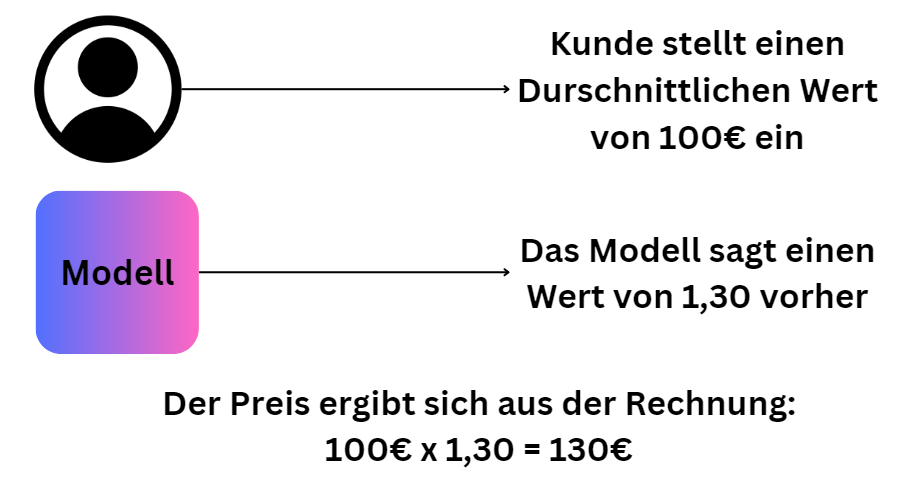
\includegraphics[width=0.5\textwidth, center]{Mitbewerber_model.png}
    \caption[Mitbewerber Modell]{Mitbewerber Modell}
    \label{img:all_hotels}
\end{figure}
